\documentclass[conference]{IEEEtran}
\IEEEoverridecommandlockouts
% The preceding line is only needed to identify funding in the first footnote. If that is unneeded, please comment it out.
\usepackage{cite}
\usepackage{amsmath,amssymb,amsfonts}
\usepackage{algorithmic}
\usepackage{graphicx}
\usepackage{textcomp}
\usepackage{xcolor}
\def\BibTeX{{\rm B\kern-.05em{\sc i\kern-.025em b}\kern-.08em
    T\kern-.1667em\lower.7ex\hbox{E}\kern-.125emX}}
\begin{document}

\title{An Efficient Wait-Free Vector in Rust}

\author{\IEEEauthorblockN{Xavier Banks}
\IEEEauthorblockA{\textit{Grad Student, Dept. Computer Science} \\
\textit{University of Central Florida}\\
Orlando, FL, USA \\
email address}
\and
\IEEEauthorblockN{Dax Borde}
\IEEEauthorblockA{\textit{Grad Student, Dept. Computer Science} \\
\textit{University of Central Florida}\\
Orlando, FL, USA \\
email address}
\and
\IEEEauthorblockN{Camilo Lozano}
\IEEEauthorblockA{\textit{Grad Student, Dept. Computer Science} \\
\textit{University of Central Florida}\\
Orlando, FL, USA \\
email address}
\and
\IEEEauthorblockN{Juan Parra}
\IEEEauthorblockA{\textit{Grad Student, Dept. Computer Science} \\
\textit{University of Central Florida}\\
Orlando, FL, USA \\
email address}
}

\maketitle

\begin{abstract}

Data structures are fundamentally important in computer science. With the introduction of new and/or popular languages, the need for data structures to natively be available arises. However, Rust being a popularized language, data structures are limited. For example, vectors are instrumental to data structures and algorithms. They are used quite frequently due to their constant-time access. There does not exist non-blocking vectors in Rust and to address this limitation, we present the first non-blocking and wait-free vector.

\end{abstract}

\begin{IEEEkeywords}
wait-free, rust, efficient, vector, concurrent
\end{IEEEkeywords}

\section{Introduction}

In today's age, applications are more complex and must perform efficiently to keep up with demand. These applications are graded upon benchmarks that result from tests. From these tests, it is well known that many applications implement some sort of algorithm to which many algorithms share common traits, these traits called data structures. These data structures are the underlying foundation to which can speed up or slow down said algorithms. For example, a vector is a container that stores a sequence of elements contiguously in memory. [1]. This allows for efficient constant-time access, rather than linear-time. However, this becomes more hazy when dealing with concurrent vectors.

Rust has become a popular language for safe multi-threaded applications as it was built from the ground up with concurrency in mind. The idea is that while writing the code it is more strictly typed than other languages it will not let you make mistakes that can commonly occur in other such languages. For example segmentation faults are hard to come by once you have some working code. 
Another benefit that Rust brings to the table is its memory management; all variables must be declared with a ‘lifetime’ which can either be implied by it’s scope or explicitly in the header of a function. In turn this allows for your code to have efficiently managed memory without really having to worry about how it gets done. In fact one of the draws of both the paper and the C++ implementation is that they do not go into detail or explain how memory is managed. One of the benchmarks of the C++ code can take up to 10 gigabytes since it is not taking care of freeing memory, presumably because of how complicated it can be to implement. If done properly our implementation will have this feature natively from the Rust implementation.
The challenge comes in a couple of parts: Rust’s strictly typed restrictions, lack of similar data structures in Rust, and the group’s unfamiliarity with the language.
Part of the reason Rust can be so thread safe is that it requires code to be much strictly typed. For example a basic data structure can’t be simply shared between threads. There is a concept of ‘ownership’ where once a data structure gets passed to another it can no longer be used outside of that scope. You can’t just create a vector and pass it to as many threads as you want. You must use a thread safe data structure that can wrap around it like an Arc that will allow you to ‘clone’ the structure. What this means for this project is that even though the goal is to port a 1:1 replica of the data structure in Rust, there just might not be an equivalent function or way of doing it.
This is not just a challenge in understating the wait free vector data structure but also implementing it in a language that the group is not familiar with. For all of us it is a first time in learning both the concepts and the complexities of the language. Rust can be unforgiving when it comes to how things can be done and implemented and it is a big obstacle figuring out how to work around those issues.

\subsection{Problem Statement}

The goal for this project is to establish a benchmark for a wait free vector data structure in C++ and Rust. Specifically we’ll be looking at the paper An Efficient Wait-Free Vector (Feldman 2016). Currently there exists a C++ implementation of the data structure that we’ll be using as our control. As far as we know there is no similar implementation that is publicly available for any type of wait free vector in Rust. With this project we seek to be able to implement the key features of the data structure into a new language. Once we have an equivalent implementation in Rust we will run tests on the two different implementations to see if there is any performance gain between the two implementations. We will be looking at speed, memory efficiency, and other attributes.

\section{Motivation}

In our research for this project it was interesting for us to find that there really were not many similar thread safe shared vectors, much less a wait free one. Not to say it is nonexistent, but for the most part it looks like Rust developers prefer to use some form of channels for sending information between threads. Rust’s package manager is called cargo, and packages are called crates. You can search and find what is available on crates.io . It was a surprise to us when we searched on there that there was no such data structure available. One of our ideas initially was to find a similar one and test our implementation against it. 
What we found when people asked online about how to implement a wait free vector is that most answers were to use already available implementation of channels. It seems that the general consensus is to use those when working in Rust. Unlike thread safe vectors, channels are natively baked into the language, and popular implementations such as Crossbeam.
Another popular available implementation is called ‘lockfree’, it offers a couple of different data structures that are lock free, one of which being a stack, it does not guarantee a wait free property. Although one of the main goals of the structure is to provide a solution to the ABA problem, which also happens to be one of the main goals of the paper our data structure is based on. 
Thus it is our goal to be able to have this data structure published on crates.io and have this implementation be another viable alternative to the more common channels. Additionally once we can then test how much more efficient channels really are in Rust than using a wait free vector (or vice versa).
While it is a good thing as our implementation is more unique this is a challenge because it will be harder to find support when it comes to implementing this solution with Rust’s idiosyncrasies as mentioned above.

\section{Related Work}

Our Rust implementation of a wait-free vector will be primary based on the wait-free vector described by Feldman et. al. in [main]. An open source C++ implementation of the vector described in Feldman et. al. [main] is available at [charles]. We will use this implementation to evaluate the performance of our Rust implementation.
Feldman et. al. [main] state that theirs is the only wait-free vector in literature at time of publication. The authors [main] also mention that the only other non-blocking vector is [lfvec], which provides a lock free guarantee, but not a wait free one. Since then, one paper [mrlock] has expanded upon the wait-free vector presented in [main]. However, Deligero et. al. [mrlock] do not attempt to maintain the non-blocking properties of the original vector, and instead use it sequentially in combination with a novel lock. While we will use this paper [mrlock] for reference and additional insights throughout this project, it is not directly useful for solving our proposed problem. Thus, the Feldman et. al. [main] vector remains the only wait-free vector in literature. 
This paper [main] additionally mentions Intel’s TBB library [tbb], which provides a concurrent vector. However, the documentation does not specify that this vector is non-blocking [tbb], and community discussions heavily indicate that all of the library’s collections are blocking [tbbcom]. Furthermore, Feldman et. al. [main] indicate that their vector and the lock free vector from Dechev et. al. [lfvec] are the only two non-blocking vectors in existence; the absence of TBB’s vector in this assertion, despite the detailed discussion of TBB in the paper [main], is conspicuous. Nonetheless, we plan to evaluate our Rust implementation by comparing its performance to the TBB vector, along with other blocking vector implementations. 

\section{Approach}

Given the difficulty of implementing an efficient wait-free vector for Rust, we divided the tasks up to accomplish this goal. The following is the breakdown:

    \begin{itemize}
        \item Reproduce the C++ results for a wait-free vector
        \item Determine API definitions for Rust Implementation
        \item Develop a testing environment to extract benchmark performances
        \item Create informal reasoning of corrections regarding the approach
        \item Compare benchmarks between the two languages
    \end{itemize}
    
    \subsection{Reproduce C++}
    
    This section is giving credit to the work of c650 on github for providing a reference point in the C++ implementation. Although the entity produced results, we decided it was best to reproduce their results for maximum precision. This was done by extrapolating the code and running several individual tests on components of the wait-free vector, such as popBack and pushBack. This gave us a starting point to what numbers we should expect after the Rust implementation was completed. While writing the code, we were not sure if the implementation will be better or worse, but as stated before, we were contributing a new data structure to the programming language. This would be provided with performance results and it would be up to the user to determine if the newly created data structure would fit their needs.

    \subsection{API Definitions}
    
    very broad summary since section {implementation} will talk more about it
    
    \subsection{Testing Environment}
    
    All code was compiled and tested in Linux environments (Ubuntu let's just say). This provided a standard across the board to avoid running into OS specific bugs or delays in compilation. 

\section{Implementation}

In this section, we go in detail in how the wait-free vector will be implemented and discuss the changes that were necessary to make. We will provide a summary and informal reasoning of correctness for each of the following operations:

    \begin{itemize}
        \item pushBack
        \item popBack
        \item valueAt
        \item insertAt
        \item eraseAt
    \end{itemize}
    
Due to Rust not using descriptors (as described in the C++ implementation), we took a different approach. 

\section{Rust Data Structure}

    \subsection{Runtime/Space Analysis}
    
    \subsection{Performance}

\section{Evaluation}

    \subsection{Rust versus C++}
    
    \subsection{Limitations}

\subsection{Figures and Tables}
\paragraph{Positioning Figures and Tables} Place figures and tables at the top and 
bottom of columns. Avoid placing them in the middle of columns. Large 
figures and tables may span across both columns. Figure captions should be 
below the figures; table heads should appear above the tables. Insert 
figures and tables after they are cited in the text. Use the abbreviation 
``Fig.~\ref{fig}'', even at the beginning of a sentence.

\begin{table}[htbp]
\caption{Table Type Styles}
\begin{center}
\begin{tabular}{|c|c|c|c|}
\hline
\textbf{Table}&\multicolumn{3}{|c|}{\textbf{Table Column Head}} \\
\cline{2-4} 
\textbf{Head} & \textbf{\textit{Table column subhead}}& \textbf{\textit{Subhead}}& \textbf{\textit{Subhead}} \\
\hline
copy& More table copy$^{\mathrm{a}}$& &  \\
\hline
\multicolumn{4}{l}{$^{\mathrm{a}}$Sample of a Table footnote.}
\end{tabular}
\label{tab1}
\end{center}
\end{table}

\begin{figure}[htbp]
\centerline{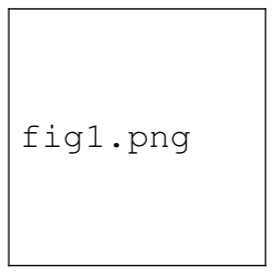
\includegraphics{fig1.png}}
\caption{Example of a figure caption.}
\label{fig}
\end{figure}

\section{Challenges}

Some of our main concerns with this is how Rust implements certain restrictions on what you can do with your objects. Granted it is meant to keep you safe from segmentation faults and other issues but it can make implementations of algorithms more complicated. Now there is a possibility that if something can’t be done in normal Rust it is possible to override some of its safety features by using a variant called unsafe Rust. Doing so would be a sort of last resort option, once you expose unsafe Rust to your code, you lose many of the guarantees that make Rust special. It allows you to access more lower level controls to the code like you would have in C++ but then you would have to provide certain guarantees to it as it is no longer safe. 
Since there are almost no other known implementations of this data structure in Rust, it also needs to be seen if it even is possible

\begin{thebibliography}{00}

% 1. ISO/IEC 14882 Standard for Programming Language C++,
% Programming languages: C++. American National Standards
% Institute, September 2011.

\bibitem{b1} G. Eason, B. Noble, and I. N. Sneddon, ``On certain integrals of Lipschitz-Hankel type involving products of Bessel functions,'' Phil. Trans. Roy. Soc. London, vol. A247, pp. 529--551, April 1955.
\bibitem{b2} J. Clerk Maxwell, A Treatise on Electricity and Magnetism, 3rd ed., vol. 2. Oxford: Clarendon, 1892, pp.68--73.
\end{thebibliography}

\end{document}
